\section{Docker Architecture}
\label{sec::arch}

% 3. Docker Architecture
%     1. The Docker engine
%         1. Client server
%         2. Monolithic architecture
%         3. runc
%         4. containerd
%     2. Images
%         1. Layers
%     3. Containers
%     4. Container creation process
%         1. Workflow
%         2. Dockerfile
%         3. Docker compose
%     5. Volumes and persistent data
%     6. Networking


\subsection{Containers}
\label{sec::arch:containers}


\subsection{The Docker Engine}
\label{sec::arch:engine}
The Docker Engine is the core software responsible for running and managing containers, which consists of several modular components following \ac{OCI} specifications\cite{Docker-engine}. It is implemented as a client-server application, consisting in the following components:

\begin{itemize}
    \item A server running the daemon process \texttt{dockerd};
    \item Docker's \acs{REST}ful \ac{API};
    \item The \ac{CLI} client, \texttt{docker}.
\end{itemize}

In this model, the Docker daemon is the component responsible for creating, running and managing the containers. The daemon is able to manage any number of containers in the device, all controlled via the \ac{CLI} interface. The client interacts with the Docker daemon via its own \ac{REST} \ac{API} over Unix sockets or a network interface\cite{Poulton2020-ju}.

\begin{figure}[!htb]
    \centering
    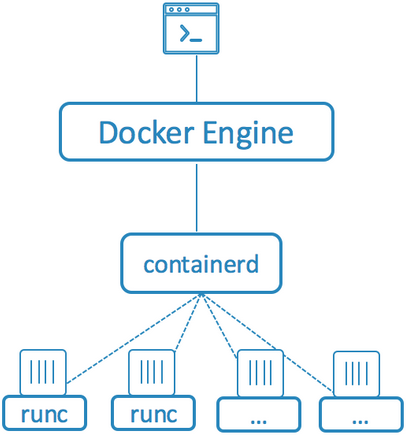
\includegraphics[width=0.25\textwidth]{docker_engine.png}
    \caption{Current and planned container use for all organizations.}
    \label{fig:docker-engine-server}
\end{figure}

Despite being at its core a client-server architecture, Docker's server is far from monolithic, as shown in figure \ref{fig:docker-engine-server}. The server operates a set of smaller components, among them \texttt{runc} and \texttt{containerd} --- the main modules responsible for creating and running containers \cite{Kane2018-fn}.

\subsubsection{\texttt{runc}}
\ac{CLI} component responsible for creating and running applications according to the \ac{OCI} runtime specifications \cite{oci-runc}, which is a open source project and available at \cite{git-runc}. Its purpose is to be a standalone low-level tool called by any high-level application, such as Docker. In order to achive this, \texttt{runc} relies on the library \texttt{libcontainer} to access the container isolation features of the \ac{OS}, such as \texttt{seccomp} and user namespaces\cite{runc-estes}.

\subsubsection{\texttt{containerd}}
Software that manages all the container execution logic, such as starting, stopping and removing containers. In the same way as \texttt{runc}, \texttt{containerd} is available as a standalone daemon and was intended to be a lightweight program with the sole role of managing container lifetime operations. But as it grew, it gained new functionalities, such as data storage and image management. \cite{docker-containerd}

% When you type commands like this into the Docker CLI, the Docker client converts
% them into the appropriate API payload and POSTs them to the correct API endpoint.
% The API is implemented in the daemon. It is the same rich, versioned, REST API that
% has become a hallmark of Docker, and is accepted in the industry as the de facto
% container API.
% Once the daemon receives the command to create a new container, it makes a call
% to containerd. Remember that the daemon no-longer contains any code to create
% containers!
% The daemon communicates with containerd via a CRUD-style API over gRPC18
% Despite its name, containerd cannot actually create containers. It uses runc to do that. It converts the required Docker image into an OCI bundle and tells runc to use this to create a new container.
% runc interfaces with the OS kernel to pull together all of the constructs necessary to create a container (namespaces, cgroups etc.). The container process is sta

\subsection{Images}
\label{sec::arch:images}


\subsubsection{Layers}

\subsection{Container Creation Process}
\label{sec::arch:cont-creation}
\subsubsection{Workflow}
\subsubsection{Dockerfile}
\subsubsection{Docker Compose}

\subsection{Volumes and Persistent Data}
\label{sec::arch:volumes}

\subsection{Networking}
\label{sec::arch:net}